% ---------------------------------------------------------------------------------------------------------------
% TEMPLATE PARA TRABALHO DE CONCLUSÃO DE CURSO
% Universidade Tecnológica Federal do Paraná - UTFPR
% Customização da classe abnTeX2 (http://www.abntex.net.br/) para as normas da UTFPR
%
% Projeto hospedado em: <link git>
% Autores: Diego Marczal  <>
% 	   Michael Vornes <https://github.com/mvornes>
%
%----------------------------------------------------------------------------------------------------------------
% Codificação: UTF-8
% LaTeX:  abnTeX2          
% ---------------------------------------------------------------------------------------------------------------


% CARREGA CLASSE PERSONALIZADA DA UTFPR--------------------------------------------------------------------------
\documentclass[%twoside,                   % Impressão em frente e verso
    	        oneside,                   % Impressão apenas frente
]{configuracoes/utfpr-abntex2}


% INCLUI ARQUIVOS DE CONFIGURAÇÕES-------------------------------------------------------------------------------
% REFERÊNCIAS------------------------------------------------------------------
\usepackage[%
    alf,
    abnt-emphasize=bf,
    bibjustif,
    recuo=0cm,
    abnt-url-package=url,       % Utiliza o pacote url
    abnt-refinfo=yes,           % Utiliza o estilo bibliográfico abnt-refinfo
    abnt-etal-cite=3,
    abnt-etal-list=3,
    abnt-thesis-year=final
]{abntex2cite}                  % Configura as citações bibliográficas conforme a norma ABNT

% PACOTES----------------------------------------------------------------------
\usepackage[utf8]{inputenc}                                 % Codificação do documento
\usepackage[T1]{fontenc}                                    % Seleção de código de fonte
\usepackage{booktabs}                                       % Réguas horizontais em tabelas
\usepackage{color, colortbl}                                % Controle das cores
\usepackage{float}                                          % Necessário para tabelas/figuras em ambiente multi-colunas
\usepackage{graphicx}                                       % Inclusão de gráficos e figuras
\usepackage{icomma}                                         % Uso de vírgulas em expressões matemáticas
\usepackage{indentfirst}                                    % Indenta o primeiro parágrafo de cada seção
\usepackage{microtype}                                      % Melhora a justificação do documento
\usepackage{multirow, array}                                % Permite tabelas com múltiplas linhas e colunas
\usepackage{subeqnarray}                                    % Permite subnumeração de equações
\usepackage{lastpage}                                       % Para encontrar última página do documento
\usepackage{verbatim}                                       % Permite apresentar texto tal como escrito no documento, ainda que sejam comandos Latex
\usepackage{amsfonts, amssymb, amsmath}                     % Fontes e símbolos matemáticos
\usepackage[algoruled, portuguese]{algorithm2e}             % Permite escrever algoritmos em português
%\usepackage[scaled]{helvet}                                % Usa a fonte Helvetica
\usepackage{times}                                          % Usa a fonte Times
%\usepackage{palatino}                                      % Usa a fonte Palatino
%\usepackage{lmodern}                                       % Usa a fonte Latin Modern
\usepackage[bottom]{footmisc}                               % Mantém as notas de rodapé sempre na mesma posição
\usepackage{ae, aecompl}                                    % Fontes de alta qualidade
\usepackage{latexsym}                                       % Símbolos matemáticos
\usepackage{lscape}                                         % Permite páginas em modo "paisagem"
%\usepackage{picinpar}                                      % Dispor imagens em parágrafos
%\usepackage{scalefnt}                                      % Permite redimensionar tamanho da fonte
%\usepackage{subfig}                                        % Posicionamento de figuras
%\usepackage{upgreek}                                       % Fonte letras gregas

% Redefine a fonte para uma fonte similar a Arial (fonte Helvetica)
\renewcommand*\familydefault{\sfdefault}

% CONFIGURAÇÕES DE APARÊNCIA DO PDF FINAL--------------------------------------
\makeatletter
\hypersetup{%
    portuguese,
    colorlinks=true,   % true: "links" coloridos; false: "links" em caixas de texto
    linkcolor=blue,    % Define cor dos "links" internos
    citecolor=blue,    % Define cor dos "links" para as referências bibliográficas
    filecolor=blue,    % Define cor dos "links" para arquivos
    urlcolor=blue,     % Define a cor dos "hiperlinks"
    breaklinks=true,
    pdftitle={\@title},
    pdfauthor={\@author},
    pdfkeywords={abnt, latex, abntex, abntex2}
}
\makeatother

% ALTERA O ASPECTO DA COR AZUL--------------------------------------------------
\definecolor{blue}{RGB}{41,5,195}

% REDEFINIÇÃO DE LABELS---------------------------------------------------------
\renewcommand{\algorithmautorefname}{Algoritmo}
\def\equationautorefname~#1\null{Equa\c c\~ao~(#1)\null}

% CRIA ÍNDICE REMISSIVO---------------------------------------------------------
\makeindex

% HIFENIZAÇÃO DE PALAVRAS QUE NÃO ESTÃO NO DICIONÁRIO---------------------------
\hyphenation{%
    qua-dros-cha-ve
    Kat-sa-gge-los
}



% INCLUI ARQUIVOS DO TRABALHO DE CONCLUSÃO DE CURSO (PRÉ-TEXTUAIS, TEXTUAIS, PÓS-TEXTUAIS)-----------------------

% INSERE CAPA E FOLHA DE ROSTO
% CAPA---------------------------------------------------------------------------------------------------

% ORIENTAÇÕES GERAIS-------------------------------------------------------------------------------------
% Caso algum dos campos não se aplique ao seu trabalho, como por exemplo,
% se não houve coorientador, apenas deixe vazio.
% Exemplos: 
% \coorientador{}
% \departamento{}

% DADOS DO TRABALHO--------------------------------------------------------------------------------------
\titulo{DISPOSITIVO VESTÍVEL PARA PROTEÇÃO INDIVIDUAL ATIVA COM MONITORAMENTO VIA WEB}
\titleabstract{Wearable device for active individual protection with WEB monitoring }
\autor{Yuri da Costa Steinmetz}
\autorcitacao{STEINMETZ, Yuri C.} % Sobrenome em maiúsculo
\local{Curitiba}
\data{2021}

% NATUREZA DO TRABALHO-----------------------------------------------------------------------------------
% Opções: 
% - Trabalho de Conclusão de Curso (se for Graduação)
% - Dissertação (se for Mestrado)
% - Tese (se for Doutorado)
% - Projeto de Qualificação (se for Mestrado ou Doutorado)
\projeto{Trabalho de Conclusão de Curso}

% TÍTULO ACADÊMICO---------------------------------------------------------------------------------------
% Opções:
% - Bacharel ou Tecnólogo (Se a natureza for Trabalho de Conclusão de Curso)
% - Mestre (Se a natureza for Dissertação)
% - Doutor (Se a natureza for Tese)
% - Mestre ou Doutor (Se a natureza for Projeto de Qualificação)
\tituloAcademico{Bacharelado em Engenharia Elétrica}

% ÁREA DE CONCENTRAÇÃO E LINHA DE PESQUISA---------------------------------------------------------------
% Se a natureza for Trabalho de Conclusão de Curso, deixe ambos os campos vazios
% Se for programa de Pós-graduação, indique a área de concentração e a linha de pesquisa
\areaconcentracao{}
\linhapesquisa{}

% DADOS DA INSTITUIÇÃO-----------------------------------------------------------------------------------
% Se a natureza for Trabalho de Conclusão de Curso, coloque o nome do curso de graduação em "programa"
% Formato para o logo da Instituição: \logoinstituicao{<escala>}{<caminho/nome do arquivo>}
\instituicao{Universidade Tecnológica Federal do Paraná}
\departamento{DAELT - DEPARTAMENTO ACADÊMICO DE ELETROTÉCNICA}
\programa{Engenharia Elétrica}
\logoinstituicao{0.2}{dados/figuras/logo-instituicao.png} 

% DADOS DOS ORIENTADORES---------------------------------------------------------------------------------
\orientador{Prof. Dr. Amauri Amorim Assef}
%\orientador[Orientadora:]{Nome da orientadora}
\instOrientador{Universidade Tecnológica Federal do Paraná}

%\coorientador{Nome do coorientador}
%\coorientador[Coorientadora:]{Nome da coorientadora}
%\instCoorientador{Instituição do coorientador}

% FOLHA DE ROSTO--------------------------------------------------------------------------------------------------------

% TRABALHO DE CONCLUSÃO DE CURSO
 \preambulo{{\imprimirprojeto} apresentado ao {\imprimirprograma} da {\imprimirinstituicao}, como requisito parcial para a obtenção do título de {\imprimirtituloAcademico}.}

% DISSERTAÇÃO DE MESTRADO
% \preambulo{{\imprimirprojeto} apresentada ao Programa de \mbox{Pós-graduação} da {\imprimirinstituicao}, como requisito parcial para obtenção do título de {\imprimirtituloAcademico}.}

% TESE DE DOUTORADO
% \preambulo{{\imprimirprojeto} apresentada ao Programa de \mbox{Pós-graduação} da {\imprimirinstituicao}, como requisito parcial para a obtenção do título de {\imprimirtituloAcademico}.}

% PROJETO DE QUALIFICAÇÃO DE MESTRADO OU DOUTORADO
%\preambulo{{\imprimirprojeto} apresentado ao Programa de \mbox{Pós-graduação} da {\imprimirinstituicao}, como requisito parcial para a obtenção do título de {\imprimirtituloAcademico}.}

% OBSERVAÇÕES-----------------------------------------------------------------------------------------------------------
% Altere este arquivo APENAS comentando as linhas que não se aplicam ao tipo de trabalho acadêmico desejado.



\begin{document}

\pretextual
\imprimircapa                                               	           % Comando para imprimir Capa
\imprimirfolhaderosto{}                                     		   % Comando para imprimir Folha de rosto
% INSERE ELEMENTOS PRÉ-TEXTUAIS
%% DEDICATÓRIA------------------------------------------------------------------

\renewcommand{\dedicatorianame}{DEDICATÓRIA}

\begin{dedicatoria}

Altere este texto inserindo a dedicatória do seu trabalho. 

\end{dedicatoria}
          			   % Dedicatória
%% AGRADECIMENTOS---------------------------------------------------------------

\begin{agradecimentos}[AGRADECIMENTOS]

Edite e coloque aqui os agradecimentos às pessoas e/ou instituições que contribuíram para a realização do trabalho.

É obrigatório o agradecimento às instituições de fomento à pesquisa que financiaram total ou parcialmente o trabalho, inclusive no que diz respeito à concessão de bolsas.

\end{agradecimentos}
        			   % Agradecimentos
%% EPÍGRAFE---------------------------------------------------------------------

\renewcommand{\epigraphname}{EPÍGRAFE}

\begin{epigrafe}

\textit{Eu denomino meu campo de Gestão do Conhecimento, mas você não pode gerenciar conhecimento. Ninguém pode. O que pode fazer - o que a empresa pode fazer - é gerenciar o ambiente que otimize o conhecimento. (PRUSAK, Laurence, 1997).}

\end{epigrafe}

% OBSERVAÇÕES------------------------------------------------------------------
% Altere o texto para inserir a epígrafe do seu trabalho

              			   % Epígrafe
% RESUMO--------------------------------------------------------------------------------

\begin{resumo}[RESUMO]
\begin{SingleSpacing}

% Não altere esta seção do texto--------------------------------------------------------
\imprimirautorcitacao. \imprimirtitulo. \imprimirdata. \pageref {LastPage} f. \imprimirprojeto\ – \imprimirprograma, \imprimirinstituicao. \imprimirlocal, \imprimirdata.\\
%---------------------------------------------------------------------------------------

O Resumo é um elemento obrigatório em tese, dissertação, monografia e TCC, constituído de uma seqüência de frases concisas e objetivas, fornecendo uma visão rápida e clara do conteúdo do estudo. O texto deverá conter no máximo 500 palavras e ser antecedido
pela referência do estudo. Também, não deve conter citações. O resumo deve ser redigido em parágrafo único, espaçamento simples e seguido das palavras representativas do conteúdo do estudo, isto é, palavras-chave, em número de três a cinco, separadas entre si por ponto e finalizadas também por ponto. Usar o verbo na terceira pessoa do singular, com linguagem impessoal, bem como fazer uso, preferencialmente, da voz ativa. Texto contendo um único parágrafo.\\

\textbf{Palavras-chave}: Palavra. Segunda Palavra. Outra palavra.

\end{SingleSpacing}
\end{resumo}

% OBSERVAÇÕES---------------------------------------------------------------------------
% Altere o texto inserindo o Resumo do seu trabalho.
% Escolha de 3 a 5 palavras ou termos que descrevam bem o seu trabalho 

             			   % Resumo em Português
% ABSTRACT--------------------------------------------------------------------------------

\begin{resumo}[ABSTRACT]
\begin{SingleSpacing}

% Não altere esta seção do texto--------------------------------------------------------
\imprimirautorcitacao. \imprimirtitleabstract. \imprimirdata. \pageref {LastPage} f. \imprimirprojeto\ – \imprimirprograma, \imprimirinstituicao. \imprimirlocal, \imprimirdata.\\
%---------------------------------------------------------------------------------------

Elemento obrigatório em tese, dissertação, monografia e TCC. É a versão do resumo em português para o idioma de divulgação internacional. Deve ser antecedido pela referência do estudo. Deve aparecer em folha distinta do resumo em língua portuguesa e seguido das palavras representativas do conteúdo do estudo, isto é, das palavras-chave. Sugere-se a elaboração do resumo (Abstract) e das palavras-chave (Keywords) em inglês; para resumos em outras línguas, que não o inglês, consultar o departamento / curso de origem.\\

\textbf{Keywords}: Word. Second Word. Another word.

\end{SingleSpacing}
\end{resumo}

% OBSERVAÇÕES---------------------------------------------------------------------------
% Altere o texto inserindo o Abstract do seu trabalho.
% Escolha de 3 a 5 palavras ou termos que descrevam bem o seu trabalho 
             		           % Resumo em Inglês
% Lista de Figuras----------------------------------------------------------------

\pdfbookmark[0]{\listfigurename}{lof}
\listoffigures*
\cleardoublepage

% OBSERVAÇÕES---------------------------------------------------------------------
% Este arquivo não precisa de ser alterado, pois a lista é gerada automaticamente.
   % Lista de Figuras
% LISTA DE QUADROS----------------------------------------------------------------

\renewcommand{\listofquadrosname}{LISTA DE QUADROS}

\pdfbookmark[0]{\listofquadrosname}{loq}
\listofquadros*
\cleardoublepage

% OBSERVAÇÕES---------------------------------------------------------------------
% Este arquivo não necessita de ser editado. A lista é gerada automaticamente.
   % Lista de Quadros
% LISTA DE TABELAS-------------------------------------------------------------

\pdfbookmark[0]{\listtablename}{lot}
\listoftables*
\cleardoublepage

% OBSERVAÇÕES-------------------------------------------------------------------
% Este arquivo não precisa ser alterado, pois a lista é gerada automaticamente.
         		   % Lista de Tabelas
% LISTA DE ABREVIATURAS E SIGLAS----------------------------------------------------------

\begin{siglas}
    \item[ABNT] Associação Brasileira de Normas Técnicas
    \item[DECOM] Departamento de Computação
\end{siglas}

% OBSERVAÇÕES-----------------------------------------------------------------------------
% Altere a lista acima para definir os acrônimos e siglas utilizados neste trabalho
          		   % Lista de Abreviaturas e Siglas
% LISTA DE SÍMBOLOS------------------------------------------------------------

\begin{simbolos}
    \item[$ \Gamma $] Letra grega Gama
    \item[$ \lambda $] Comprimento de onda
    \item[$ \in $] Pertence
\end{simbolos}

% OBSERVAÇÕES-------------------------------------------------------------------
% Altere a lista acima para definir os símbolos utilizados no trabalho
        		   % Lista de Símbolos
% LISTA DE ALGORITMOS----------------------------------------------------------

\newcommand{\algoritmoname}{Algoritmo}
\renewcommand{\listalgorithmcfname}{LISTA DE ALGORITMOS}

\floatname{algocf}{\algoritmoname}
\newlistof{listofalgoritmos}{loa}{\listalgoritmoname}
\newlistentry{algocf}{loa}{0}

\counterwithout{algocf}{chapter}
\renewcommand{\cftalgocfname}{\algoritmoname\space}
\renewcommand*{\cftalgocfaftersnum}{\hfill--\hfill}

\pdfbookmark[0]{\listalgorithmcfname}{loa}
\listofalgorithms
\cleardoublepage

% OBSERVAÇÕES------------------------------------------------------------------
% Este arquivo não precisa ser alterado, pois a lista é gerada automaticamente.
   % Lista de Algoritmos
% SUMÁRIO----------------------------------------------------------------------

\renewcommand{\contentsname}{SUMÁRIO}

\pdfbookmark[0]{\contentsname}{toc}
\tableofcontents*
\cleardoublepage

% OBSERVAÇÕES-------------------------------------------------------------------
% Este arquivo não precisa ser alterado, pois o sumário é gerado automaticamente.
               			   % Sumário

\textual
% INSERE ELEMENTOS TEXTUAIS
% INTRODUÇÃO-------------------------------------------------------------------

\chapter{INTRODUÇÃO}
\label{chap:introducao}

Acidentes de trabalho causam problemas incalculáveis tanto para o trabalhador, quanto para a empresa que possui perdas de ativos tangíveis, intangíveis e capital humano. O Brasil tem sido um dos países que mais sofrem com esse importante problema, onde ocorreu, neste século, um acidente de trabalho fatal a cada duas horas e meia, conforme Mattos (2011).  O autor complementa que nos países em desenvolvimento 10 do produto interno bruto (PIB) é perdido devido a doenças e agravos ocupacionais que além da morte e de sofrimento para o trabalhador e para sua família, problemas ainda pouco estudados, os acidentes de trabalho têm reflexos socioambientais, econômicos e políticos para toda a sociedade.
O Tribunal de Justiça do Trabalho, define acidente de trabalho, no artigo 19 da Lei nº 8.213 de 1991, como:

\begin{citacao}
Acidente de trabalho é o que ocorre pelo exercício do trabalho a serviço da empresa ou pelo exercício do trabalho dos segurados referidos no inciso VII do art. 11 desta lei, provocando lesão corporal ou perturbação funcional que cause a morte ou a perda ou redução, permanente ou temporária, da capacidade para o trabalho. Ao lado da conceituação acima, acedente de trabalho típico, por expressa determinação legas, as doenças profissionais e/ou ocupacionais equiparam-se a acidentes de trabalho. (TRIBUNAL DE JUSTIÇA DO TRABALHO, 2020). 
\end{citacao}

Há muito tempo já existia relatos de doenças relacionadas as atividades laborais, pelos Egípcios, Babilônicos e greco-romanos. Há relatos de registros Egípcios relacionando acidentes de trabalho e os riscos inerentes às atividades datadas de 2360 a.C, primeiramente, relacionado a uma premissa mágico-religiosa e, posteriormente, numa perspectiva naturalista (MATTOS, 2011).
Mostrando que são problemas antigos e por muitas vezes inerentes à atividade exercida pelo indivíduo, Mattos (2011) contextualiza alguns acontecimentos relatados pelo povo Grego, sendo eles os responsáveis pela mudança do paradigma espiritualista para o naturalista. Como exemplo, Hipócrates descreveu a intoxicação saturnina, porém sem descrever o ambiente e a ocupação laboral. Plínio, o Velho (23-79 a.C.), relatou em seu trabalho, o tratado História Naturalis, o aspecto de trabalhadores expostos ao chumbo, mercúrio e poeiras, descrevendo os primeiros equipamentos de proteção individual (EPIs), sendo estas máscaras feitas de pano e bexigas.
Os autores Barsano e Barbosa (2012) descrevem algumas premissas das condições de trabalho de forma evitar acidentes e otimizar o nível de segurança dos trabalhadores:

\begin{citacao}
Portanto, no ambiente de trabalho necessitamos encontrar condições capazes de proporcionar o máximo de proteção e ao mesmo tempo satisfação no trabalho. E quando existe essa combinação, com toda certeza resulta num aumento significativo da produtividade, melhoria da qualidade dos serviços, redução do índice de absenteísmo e diminuição drástica das doenças e dos acidentes do trabalho. (BARSANO; BARBOSA, 2012). 
\end{citacao}

\section{TEMAS DE PESQUISA}
\label{sec:temasDePesquisa}

Mensurar e supervisionar a exposição a ambientes insalubres conforme a Norma Regulamentadora (NR) 15, Atividades e Operações Insalubres (MINISTÉRIO DO TRABALHO E EMPREGO, 2007), pois segundo Barsano e Barbosa (2012): quando um desses fatores, ou um conjunto deles, foge ao controle, seja pelos níveis permitidos ou pelos processos que se desencadeiam, o ambiente de trabalho torna-se suscetível de desenvolver as chamadas patologias do trabalho. Estes agentes são descritos na NR 9 (MINISTÉRIO DO TRABALHO E EMPREGO, 1978) em três categorias: físicos, químicos e biológicos. 

\section{DELIMITAÇÃO DE PESQUISA}
\label{sec:delimitacaoDePesquisa}

Nesta pesquisa, alguns agentes físicos serão avaliados, sendo que a NR 9 descreve os agentes físicos, como: ruídos, vibrações, pressões anormais, temperaturas extremas, radiações ionizantes, radiações não ionizantes, bem como o infrassom e ultrassom.
Os agentes físicos que estão em foco deste Trabalho de Conclusão de Curso (TCC) são: ruídos, vibrações, temperaturas e radiações não ionizantes (luz), que podem ser facilmente mensurados e comparados com os valores estabelecidos na norma NR 15, de forma a ter um melhor controle sob a exposição e prevenido as patologias, sendo mensurados por sensores de baixa complexidade e podendo ser embarcado em dispositivo vestível de baixo custo.

\section{PROBLEMÁTICA E PREMISSAS DE PESQUISA}
\label{sec:problematicaEPremissasDePesquisa}

De acordo com Lusk et al. (apud MEIRA et al, 2012): “O ruído causa vários efeitos indesejáveis à saúde dos indivíduos expostos, como zumbido, aumento da pressão arterial e da frequência cardíaca, insônia, estresse e irritabilidade”.
A exposição à vibração ocupacional, gera diversos danos à saúde do trabalhador como doenças vasculares, neurológicas e musculares. Cristiano Molica (2018), em entrevista ao PodPrevenir, descreve que “uma vibração de alta amplitude nas mãos por exemplo, gera uma síndrome chamada síndrome do dedo branco que afeta todo o sistema circulatório podendo até gerar amputação do membro superior”. 
A exposição ao calor causa brotoejas, câimbras, exaustão e insolação; com os sintomas de que o corpo precisa ser resfriado sendo: dor de cabeça, fraqueza, suor excessivo, irritabilidade ou confusão mental, sede, náuseas e vômitos diz a fabricante de EPIs Dupont (2019) em seu blog.
Lorenzi (2020) lista as doenças causadas pela má iluminação, sendo elas: irritação dos olhos, cansaço visual, distúrbios emocionais e problemas de pele.
Os ambientes de trabalho são lugares dinâmicos e muito complexos. Apenas os fatores descritos acima já influenciam uma quantidade considerável de pessoas nas áreas de manufatura de produtos e beneficiamento de alimentos, saúde, escritórios e outros tipos de serviços. Sendo assim, as normas e procedimentos atuais realmente são suficientes para garantir que todos esses colaboradores estão protegidos dessas enfermidades?
A mensuração constante, controle automático e supervisão desses parâmetros mesmo que não seja feita com instrumentos precisos desenvolvidos para tal, podem indicar a magnitude e dar uma ideia de pontos a serem observados com mais cuidado.

\section{OBJETIVOS DA PESQUISA}
\label{sec: objetivosDaPesquisa}

\subsection{Objetivo Geral}
\label{sec: objetivoGeral}

Desenvolver um sistema embarcado composto de um dispositivo vestível com sensores de temperatura, vibração e ruído com capacidade de transferência de dados para um servidor WEB de supervisão e monitoramento. 

\subsection{Objetivos Específicos}
\label{sec: objetivoEspecificos}

\begin{itemize}
    \item   Selecionar os sensores.
    \item	Integrar os sensores ao sistema microcontrolador.
    \item	Desenvolver o circuito embarcado.
    \item	Desenvolver o firmware.
    \item	Desenvolver o servidor.
    \item	Desenvolver a aplicação WEB.
    \item	Integrar o dispositivo e a aplicação ao servidor.

\end{itemize}

\section{JUSTIFICATIVA}
\label{sec: justificativa}

Um acidente não ocorre por uma única causa, mas sim por uma série de fatores contribuintes.

\begin{citacao}
A abordagem holística da segurança do trabalho é outra forma em que visualizamos os acidentes. Nela não afirmamos que o acidente teve uma única e exclusiva origem, mas foi gerado pela interação simultânea de diversos fatores (físicos, biológicos, psicológicos, sociais e culturais), e que um desencadeou o outro, gerando um acidente. Logo não há uma causa única dos acidentes, e sim várias. (BARSANO e BARBOSA, 2018, p. 24). 
\end{citacao}

Lito Sousa (2015) destaca que as capacidades humanas se deterioram com a complacência e que cada vez mais a ciência e a tecnologia trabalham para que os erros diminuam e na impossibilidade de eliminá-los, que seus efeitos não causem um acidente grave ou fatal.
A aviação trabalha a partir do fato de que seres humanos são falhos e por isso dispõem de diversas camadas de proteção contra acidentes. Souza (2009) expõem que por vezes a mente pode criar uma falsa memória baseada em experiências anteriores, ou seja, um procedimento de segurança pode ser esquecido pois o cérebro pode ter injetado a memória de ter executado aquela tarefa a partir da memória de centenas de execuções posteriores.
Dado os altos números de acidentes destacado no início deste trabalho e as limitações do ser humano, surge a percepção inspirada na aviação da necessidade de mais camadas de segurança para combater os altos números supra citados, uma camada com base na tecnologia que reduza os erros decorrentes do homem, colete dados, tome ações de controle e supervisione o dia a dia do trabalhador. 

\section{PROCEDIMENTOS METODOLÓGICOS}
\label{sec: procedimentosMetodologicos}

O trabalho inicia-se com a consulta à NR 9 sobre os limites de exposição aos agentes físicos. Desta forma, poder-se-á ter uma noção da escala, acurácia e precisão dos sensores. Assim, a próxima etapa é a escolha dos sensores com base nos requisitos e facilidade de implementação.
Dando início ao processo de prototipagem do dispositivo de forma que seja vestível e tenha embarcado cada um dos sensores, será realizado o desenvolvimento do firmware para a correta leitura das grandezas a serem medidas, transmissão destes dados ao servidor e emissão de alertas ao usuário.
O próximo passo é o desenvolvimento do servidor que receberá os dados e registra os avisos de forma que seja visível aos gestores. Seguido dos testes de hardware, firmware e software. 
Por fim, serão obtidos os resultados para a última etapa, na qual será feita a análise do sistema para se concluir se o dispositivo obteve êxito e também o registro dos principais pontos de aprendizado.


\section{ESTRUTURA}
\label{sec: estrutura}

Este trabalho será composto por seis capítulos: o primeiro será uma abordagem do tema, sua delimitação, as problemáticas, objetivos, justificativa e descrição dos procedimentos metodológicos adotados. No segundo capítulo será feita uma revisão bibliográfica. O terceiro é apresentado a proposta do sistema e do dispositivo. No quarto será discutido os detalhes de implementação e as tecnologias dos sensores, acumuladores de energia, comunicação, sistemas microcontrolados. Também será discutida as tecnologias empregadas no servidor e na aplicação WEB. No quinto capítulo será discutido o desenvolvimento e implementação do sistema. O último será discutido os resultados obtidos a partir de testes em ambiente controlado do dispositivo. 

\section{CRONOGRAMA}
\label{sec: cronograma}

O trabalho será desenvolvido em um período de três semestres letivos com cada etapa sendo detalhada na...

                		           % Introdução
% REVISÃO DE LITERATURA--------------------------------------------------------

\chapter{FUNDAMENTAÇÃO TEÓRICA}
\label{chap:fundamentacaoTeorica}

\section{SENSORES}
\label{sec:sensores}

Sensores, no contexto da engenharia elétrica é a conversão de grandezas físicas em grandezas elétricas que então podem ser interpretadas através de displays no corpo do instrumento de medida ou então enviadas a outro dispositivo para ser processada. “Utilizam-se os efeitos físicos (força eletromagnética, força eletrostática, efeito Joule, efeito termoelétrico, entre outros) para fornecer esses dados aos instrumentos através de grandezas elétricas”. 

\section{DETECÇÃO DE LUZ}
\label{subsec:detecaoDeLuz}

Para detectar o nível de luminosidade do local um dispositivo fotocondutor chamado de resistor LDR (do inglês light dependent resistor) pode ser usado. Este quando exposto à luz possui uma baixa resistência e possui comportamento contrário quando longe de quaisquer fontes luminosas.

Podemos detectar essas variações de sua resistência indiretamente através do uso de um divisor resistivo, onde o LDR será inserido em série com um resistor com valor conhecido. Segundo Kilari et al (2020), o desempenho desta solução é semelhante a Luxímetros comerciais tendo um desempenho muito próximo de um valor linear.

Esse comportamento é explicado por Balbinot (2019), onde a exposição à luz resulta em elétron livre que é deslocado da banda de valência para a de condução assim quando exposto à um potencial elétrico ocasiona o movimento de elétrons e lacunas.

\section{SENSOR DE VIBRAÇAO}
\label{subsec:sensorDeVibracao}

Os autores supracitados destacam que os danos causados pela vibração dependem da média da aceleração a qual a região está exposta durante um dia de trabalho. Eles também apresentam os seguintes dados a respeito dos efeitos de vibrações no corpo humano de acordo com cada faixa de frequência sendo:

\begin{citacao}
Na atividade muscular, na faixa de 1 Hz a 30 Hz, as pessoas apresentam dificuldades de manter a postura, além de apresentar reflexos lentos; no sistema cardiovascular, a frequências inferiores a 20 Hz, observa-se aumento da frequência cardíaca; 	aparentemente existem alterações nas condições de ventilação pulmonar e na taxa respiratória com vibrações na ordem de 4,9 m/s2 na faixa de 1 Hz a 10 Hz; 	na faixa de frequência de 0,1 Hz a 0,7 Hz, diversas pessoas apresentam enjoo, náuseas, perda de peso, redução da acuidade visual, insônia e distúrbios do labirinto 
\end{citacao}

Para medir vibrações nestas frequências foi selecionado o acelerômetro capacitivo que segundo Balbinot (2019) tem uma vantagem sobre os acelerômetros piezo resistiva por permitirem medir inclinações de objetos em relação a sua superfície.

Seu funcionamento em Figura 2 é descrito pelo autor como dois capacitores diferenciais com uma placa central comum representada na figura acima pela cor azul. A placa comum é presa a uma viga móvel que se encontra sustentada por outras duas paredes flexíveis representadas em amarelo. Quando o dispositivo é submetido a aceleração a viga se desloca movimentando consigo a placa comum e assim provocando uma diferença de capacitância.

No caso deste trabalho, considere a figura 3, o uso de acelerômetro capacitivo nos permite detectar o ângulo do braço do usuário e assim distinguir movimentos de vibrações, uma vez que as vibrações do uso de ferramentas oscilaram em torno do ângulo de trabalho do operador.

\section{SENSOR DE VIBRAÇÃO}
\label{subsec: sensorDeVibracao}

O que é o som? Segundo Balbinot (2019) sua definição é qualquer oscilação de pressão, seja no ar, água ou qualquer outro meio físico. Ou formalmente é a diferença entre a pressão instantânea e a pressão ambiente média para certo ponto definida como:

\begin{citacao}
Na atividade muscular, na faixa de 1 Hz a 30 Hz, as pessoas apresentam dificuldades de manter a postura, além de apresentar reflexos lentos; no sistema cardiovascular, a frequências inferiores a 20 Hz, observa-se aumento da frequência cardíaca; 	aparentemente existem alterações nas condições de ventilação pulmonar e na taxa respiratória com vibrações na ordem de 4,9 m/s2 na faixa de 1 Hz a 10 Hz; 	na faixa de frequência de 0,1 Hz a 0,7 Hz, diversas pessoas apresentam enjoo, náuseas, perda de peso, redução da acuidade visual, insônia e distúrbios do labirinto 
\end{citacao}

Para medir vibrações nestas frequências foi selecionado o acelerômetro capacitivo que segundo Balbinot (2019) tem uma vantagem sobre os acelerômetros piezo resistiva por permitirem medir inclinações de objetos em relação a sua superfície.

Seu funcionamento em Figura 2 é descrito pelo autor como dois capacitores diferenciais com uma placa central comum representada na figura acima pela cor azul. A placa comum é presa a uma viga móvel que se encontra sustentada por outras duas paredes flexíveis representadas em amarelo. Quando o dispositivo é submetido a aceleração a viga se desloca movimentando consigo a placa comum e assim provocando uma diferença de capacitância.

No caso deste trabalho, considere a figura 3, o uso de acelerômetro capacitivo nos permite detectar o ângulo do braço do usuário e assim distinguir movimentos de vibrações, uma vez que as vibrações do uso de ferramentas oscilaram em torno do ângulo de trabalho do operador.


\section{SENSOR DE SOM}
\label{subsec: sensorDeSom}

O que é o som? Segundo Balbinot (2019) sua definição é qualquer oscilação de pressão, seja no ar, água ou qualquer outro meio físico. Ou formalmente é a diferença entre a pressão instantânea e a pressão ambiente média para certo ponto definida como:

Santini et al, possuem uma definição para pressão sonora levando em consideração um intervalo de tempo, o valor rms (root mean square) do valor da pressão instantânea e o mínimo audível pelo ser humano:

Os principais efeitos no corpo humano de ruídos quando ultrapassam limites estabelecidos em norma são: “mascaramento da voz humana, surdez temporária, surdez permanente irregularidade do sono e aumento da pressão arterial” (BALBINOT, 2019).

Para medir essas variações de pressão no ar o microfone omnidirecional condensador (ou capacitivo) pode ser utilizado por possuir baixa distorção e alta estabilidade, seu funcionamento é descrito pelo autor citado anteriormente e consiste de um diafragma montado a uma pequena distância de um prato e ambos formam um capacitor, quando o diafragma é submetido a algum diferencial de pressão ele se move alterando a distância de si mesmo e o prato gerando um diferencial de reatância.

\section{SENSOR DE TEMPERATURA}
\label{subsec: sensorDeTemperatura}

A matéria muda algumas de suas características quando submetida a diferentes variações de temperatura, o que não poderia ser diferente para os semicondutores tais como diodos e transistores. Devido à miniaturização dos semicondutores tornou-se fácil o seu uso em dispositivos vestíveis Balbinot (2019) descrevem como podemos utilizar transistores para medir temperatura. 
Semicondutores são isolantes a baixas temperaturas, porém sua condutividade aumenta junto com o fornecimento de calor a ele, portanto teoricamente podemos utilizar um diodo para tal, mas a variação de condutividade não é linear a variação de temperatura além de que a corrente que passa por ele também é dependente da temperatura. Outra possibilidade seria utilizar um transistor e utilizar a dependência com a temperatura da tensão base-emissor, porém para isso é necessária uma fonte de corrente contínua levando a seguinte solução apresentada pelos autores:

O circuito apresentado acima é popularmente conhecido como conversor de temperatura-corrente e é amplamente utilizado nos circuitos integrados. Os transistores Q3 e Q4 são idênticos resultando em correntes de mesma magnitude passando por eles, o transistor Q2 é um arranjo de 8 transistores em paralelo sendo cada um deles idênticos a Q1 de forma que a corrente no emissor de um transistor de Q2 é 1/8 a corrente de Q1. Tomando o resistor R igual a 358 Ω temos a seguinte equação:

\section{LIMITES DE ESPOSIÇÃO ESTABELECIDOS EM NORMA}
\label{subsec: sensorDeEsposicaoEstabelecidosEmNorma}

O ambiente de trabalho possui agentes físicos que interfere na saúde humana. Para que estes agentes não gerem danos a NR 9 estabeleceu limites de tolerância relacionados com a natureza e o tempo de exposição a fim de não causar danos a saúde do trabalhador.


\begin{table}[]
    \centering
    \begin{tabular}{ | l | l | }
\hline
	NÍVEL DE RUÍDO dB (A) & MÁXIMA EXPOSIÇÃO DIÁRIA PERMISSÍVEL (horas) \\ \hline
	85 & 8 horas \\ 
	86 & 7 horas \\ 
	87 & 6 horas \\ 
	88 & 5 horas \\ 
	89 & 4 horas e 30 minutos \\ 
	90 & 4 horas \\ 
	91 & 3 horas e 30 minutos \\ 
	92 & 3 horas \\
	93 & 2 horas e 40 minutos \\ 
	94 & 2 horas e 15 minutos \\
	95 & 2 horas \\
	96 & 1 hora e 45 minutos \\
	98 & 1 hora e 15 minutos \\
	100 & 1 hora \\
	102 & 45 minutos \\
	104 & 35 minutos \\
	105 & 30 minutos \\
	106 & 25 minutos \\
	108 & 20 minutos \\ 
	110 & 15 minutos \\ 
	112 & 10 minutos \\ 
	114 & 8 minutos \\
	115 & 7 minutos \\ \hline
\end{tabular}
    \caption{Limites de tolerância para ruído contínuo ou intermitente}
    \label{tab:limitesDeTolerancia}
\end{table}

Caso o ruído seja do tipo de impacto, definido pela NR 9 como: “Entende-se por ruído de impacto aquele que apresenta picos de energia acústica de duração inferior a 1 (um) segundo, a intervalos superiores a 1 (um) segundo”. Para este caso deve-se usar a tabela 3 - Níveis de pico máximo admissíveis em função do número de impactos.

\section{VIBRAÇÃO}
\label{subsec: vibracao}

A NR 9 estabelece que o limite máximo de exposição diária à vibração em mãos e braços é medido em aceleração resultante de exposição normalizada (aren) e deve ser de no máximo 5 m/s2. Cabe a Fundacentro definir como são calculados esses limites, sendo a aren é calculada por:

\begin{itemize}
    \item are é a aceleração resultante de exposição.
    \item T é o tempo de duração da jornada de trabalho diária.
    \item 	T0 é igual a 8 horas.
\end{itemize}

A aceleração resultante é calculada utilizando-se outras duas medidas sendo a primeira a aceleração média resultante (amr) que consiste de uma média aritmética das acelerações em cada componente do sistema tridimensional. A medida necessária é a aceleração resultante de exposição parcial (arep) que pode ser obtido pela média aritmética da aceleração média resultante cada vez em que ocorre uma aceleração no eixo em que estamos observando a vibração.
Para calcular a aceleração resultante de exposição a seguinte formula deve ser usada:

Sendo que:

\begin{itemize}
    \item arep é a aceleração resultante de exposição parcial.
    \item n é o número de repetições ao longo da jornada de trabalho.
    \item m representa i, j e k que correspondem aos eixos x, y e z respectivamente.
\end{itemize}

\section{TEMPERATURA}
\label{subsec: temperatura}

A NR 9 estabelece limites a exposição ao calor, segundo a mesma o limite de temperatura varia conforme a atividade exercida pois cada atividade possui uma taxa metabólica. Como a tabela é demasiadamente grande para este trabalho apenas consideraremos as seguintes atividades: trabalho sentado leve com as mãos, trabalho sentado pesado com dois braços, trabalho em pé com movimento sem carga a 4 km/h.

Para essas atividades a temperatura máxima deve seguir a seguindo a tabela 5.

\section{LUMINOSIDADE}
\label{subsec: luminosidade}

A ABNT NBR ISO/CIE 8995-1 estabelece os parâmetros de iluminação que um ambiente deve obedecer. Neste trabalho apenas vamos conseguir medir a iluminância do ambiente através de um resistor LDR, cada ambiente tem um valor mínimo estabelecido na norma porém vamos considerar apenas um local de usinagem onde a iluminância média mínima deve ser de 300 lux.

\section{COMO AS PÁGINAS WEB FUNCIONAM}
\label{sec: como as paginas web funcionam}

\section{HTML}
\label{subsec: html}

O HTML (hypertext marking language) nas palavras da Mozilla (2021) é o bloco de construção da internet. Ela diz ao navegador onde cada elemento deve estar e como ele deve ser estruturado ao usuário. Ele envolve o conteúdo entre tags para que ele haja de uma certa maneira, para envolver o conteúdo temos a seguinte estrutura <(nome da tag)>  texto </(nome da tag)> e tudo o que estiver entre elas se comporta conforme suas características, por exemplo considere as seguintes tags:

\begin{itemize}
    \item h1 - Cria um título.
    \item p - Cria um parágrafo.
    \item ul - Cria uma lista não numerada.
    \item li - Adiciona elementos a lista.
\end{itemize}


Existem inúmeras outras tags HTML que podem ser consultadas em sua documentação oficial. Para construir uma lista de compras, por exemplo, podemos apenas envolver nossa lista entre estas tags da seguinte forma: <h1>Lista de compras</h1><p>Itens básicos que estão faltando em casa:</p><ul><li>Maçã</li><li>Laranja</li><li>Pera</li>.

\section{CSS}
\label{subsec: html}

É a abreviação de (Cascading Style Sheets) e de acordo com a organização citada anteriormente ela é responsável por dar estilo ao HTML e é um padrão adotado em todos os navegadores. Por exemplo, para mudar a cor do título de nossa lista basta escrever a tag h1 da seguinte forma: <h1 style="color:red">Lista de compras</h1>.

\section{PHP}
\label{subsec: php}

Segundo o site dos desenvolvedores do PHP (Hypertext Preprocessor) é uma linguagem de script que é inserido entre o código HTML o dando a capacidade de rodar scripts, estes scripts são processados inteiramente do lado do servidor, podendo gerar páginas dinâmicas com base nos dados recebidos de um método HTTP (o HTTP será discutido futuramente). Um dos exemplos de uma aplicação do PHP é uma tela de login em um sistema, ao preenchermos nossas credenciais e ao clicar em enviar o servidor processa os dados recebidos e nos retorna uma nova página.

\section{PHP}
\label{subsec: php}

Segundo o site dos desenvolvedores do PHP (Hypertext Preprocessor) é uma linguagem de script que é inserido entre o código HTML o dando a capacidade de rodar scripts, estes scripts são processados inteiramente do lado do servidor, podendo gerar páginas dinâmicas com base nos dados recebidos de um método HTTP (o HTTP será discutido futuramente). Um dos exemplos de uma aplicação do PHP é uma tela de login em um sistema, ao preenchermos nossas credenciais e ao clicar em enviar o servidor processa os dados recebidos e nos retorna uma nova página.

         % Revisão de Literatura
% METODOLOGIA------------------------------------------------------------------

\chapter{METODOLOGIA}
\label{chap:metodologia}
Cada capítulo deve conter uma pequena introdução (tipicamente, um ou dois parágrafos) que deve deixar claro o objetivo e o que será discutido no capítulo, bem como a organização do capítulo.

\section{DELINEAMENTO DA PESQUISA}
\label{sec:titSecDelPesq}

Inserir seu texto aqui...

\section{COLETA E TRATAMENTO DE DADOS}
\label{sec:titSecColDad}

Inserir seu texto aqui...

                   % Metodologia
% RESULTADOS-------------------------------------------------------------------

\chapter{ANÁLISE E DISCUSSÃO DOS RESULTADOS}

Cada capítulo deve conter uma pequena introdução (tipicamente, um ou dois parágrafos) que deve deixar claro o objetivo e o que será discutido no capítulo, bem como a organização do capítulo.
                    % Resultados
% ORIENTAÇÕES GERAIS------------------------------------------------------------


% SOBRE AS ILUSTRAÇÕES----------------------------------------------------------
\chapter{SOBRE AS ILUSTRAÇÕES}
\label{chap:apSobreIlust}

A seguir exemplifica-se como inserir ilustrações no corpo do trabalho. As ilustrações serão indexadas automaticamente em suas respectivas listas. A numeração sequencial de figuras, tabelas e equações também ocorre de modo automático.

Referências cruzadas são obtidas através dos comandos \verb|\label{}| e \verb|\ref{}|. Sendo assim, não é necessário por exemplo, saber que o número de certo capítulo é \ref{chap:fundamentacaoTeorica} para colocar o seu número no texto. Outra forma que pode ser utilizada é esta: \autoref{chap:fundamentacaoTeorica}, facilitando a inserção, remoção e manejo de elementos numerados no texto sem a necessidade de renumerar todos esses elementos.

% FIGURAS-----------------------------------------------------------------------
\chapter{FIGURAS}
\label{chap:figuras}

Exemplo de como inserir uma figura. A \autoref{fig:figura-exemplo1} aparece automaticamente na lista de figuras. Para saber mais sobre o uso de imagens no \LaTeX{} consulte literatura especializada \cite{Goossens2007}.

Os arquivos das figuras devem ser armazenados no diretório de "/dados".

\begin{figure}[!htb]
    \centering
    \caption{Exemplo de Figura}
    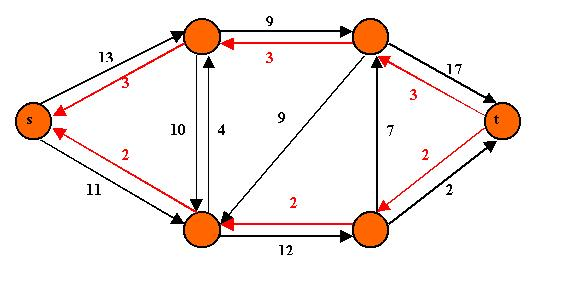
\includegraphics[width=0.5\textwidth]{./dados/figuras/figura1}
    \fonte{\citeonline{IRL2014}}
    \label{fig:figura-exemplo1}
\end{figure}

% QUADROS E TABELAS---------------------------------------------------------------
\chapter{QUADROS E TABELAS}
\label{chap:tabelas}

Exemplo de como inserir o \autoref{qua:quadro-exemplo1} e a \autoref{tab:tabela-exemplo1}. Ambos aparecem automaticamente nas suas respectivas listas. Para saber mais informações sobre a construção de tabelas no \LaTeX{} consulte literatura especializada \cite{Mittelbach2004}.

Ambos os elementos (Quadros e Tabelas) devem ser criados em arquivos separados para facilitar manutenção e armazenados no diretório de "/dados".

\begin{quadro}[!htb]
    \centering
    \caption{Exemplo de Quadro.\label{qua:quadro-exemplo1}}
    \begin{tabular}{|p{7cm}|p{7cm}|}
        \hline
        \textbf{BD Relacionais} & \textbf{BD Orientados a Objetos} \\
        \hline
        Os dados são passivos, ou seja, certas operações limitadas podem ser automaticamente acionadas quando os dados são usados. Os dados são ativos, ou seja, as solicitações fazem com que os objetos executem seus métodos. & Os processos que usam dados mudam constantemente. \\
        \hline
    \end{tabular}
    \fonte{\citeonline{Barbosa2004}}
\end{quadro}


A diferença entre quadro e tabela está no fato que um quadro é formado por linhas horizontais e verticais. Deve ser utilizado quando o conteúdo é majoritariamente não-numérico. O número do quadro e o título vem acima do quadro, e a fonte, deve vir abaixo. E Uma tabela é formada apenas por linhas verticais. Deve ser utilizada quando o conteúdo é majoritariamente numérico. O número da tabela e o título vem acima da tabela, e a fonte, deve vir abaixo, tal como no quadro.

\begin{table}[!htb]
    \centering
    \caption[Resultado dos testes]{Resultado dos testes.
    \label{tab:tabela-exemplo1}}
    \begin{tabular}{rrrrr}
        \toprule
            & Valores 1 & Valores 2 & Valores 3 & Valores 4 \\
        \midrule
            Caso 1 & 0,86 & 0,77 & 0,81 & 163 \\
            Caso 2 & 0,19 & 0,74 & 0,25 & 180 \\
            Caso 3 & 1,00 & 1,00 & 1,00 & 170 \\
        \bottomrule
    \end{tabular}
    \fonte{\citeonline{Barbosa2004}}
\end{table}


\begin{table}[!htb]
    \centering
    \caption[Cronograma]{Cronograma.
    \label{tab:cronograma}}
    \begin{tabular}{rrrrr}
        \toprule
            & Fases/ano de pesquisa & 2020 & 2021 \\
        \midrule
            Meses & ago & set & out &  \\
            Caso 2 & 0,19 & 0,74 & 0,25 & 180 \\
            Caso 3 & 1,00 & 1,00 & 1,00 & 170 \\
        \bottomrule
    \end{tabular}
    \fonte{\citeonline{Barbosa2004}}
\end{table}

% EQUAÇÕES-----------------------------------------------------------------------
\chapter{EQUAÇÕES}
\label{chap:equacoes}

Exemplo de como inserir a \autoref{eq:equacao-exemplo1} e a Eq. \ref{eq:equacao-exemplo2} no corpo do texto \footnote{Deve-se atentar ao fato de a formatação das equações ficar muito boa esteticamente.}. Observe que foram utilizadas duas formas distintas para referenciar as equações.

\begin{equation}
    X(s) = \int\limits_{t = -\infty}^{\infty} x(t) \, \text{e}^{-st} \, dt
    \label{eq:equacao-exemplo1}
\end{equation}

\begin{equation}
    F(u, v) = \sum_{m = 0}^{M - 1} \sum_{n = 0}^{N - 1} f(m, n) \exp \left[ -j 2 \pi \left( \frac{u m}{M} + \frac{v n}{N} \right) \right]
    \label{eq:equacao-exemplo2}
\end{equation}

% ALGORITMOS-----------------------------------------------------------------------
\chapter{ALGORITMOS}
\label{chap:algoritmos}

Exemplo de como inserir um algoritmo. Para inserção de algoritmos utiliza-se o pacote {\ttfamily algorithm2e} que já está devidamente configurado dentro do template.

Os algoritmos devem ser criados em arquivos separados para facilitar manutenção e armazenados no diretório de "/dados".\\
\\

\begin{algorithm}
    \caption{Exemplo de Algoritmo}
    \KwIn{o número $n$ de vértices a remover, grafo original $G(V, E)$}
    \KwOut{grafo reduzido $G'(V,E)$}
    $removidos \leftarrow 0$ \\
    \While {removidos $<$ n } {
        $v \leftarrow$ Random$(1, ..., k) \in V$ \\
            \For {$u \in adjacentes(v)$} {
                remove aresta (u, v)\\
                $removidos \leftarrow removidos + 1$\\
            }
            \If {há  componentes desconectados} {
                remove os componentes desconectados\\
            }
        }
\end{algorithm}


% SOBRE AS LISTAS--------------------------------------------------------------------
\chapter{SOBRE AS LISTAS}
\label{chap:apSobreLista}

Para construir listas de "\textit{bullets}"{} ou listas enumeradas, inclusive listas aninhadas, é utilizado o pacote \verb|paralist|.

Exemplo de duas listas não numeradas aninhadas, utilizando o comando \verb|\itemize|. Observe a indentação, bem como a mudança automática do tipo de "\textit{bullet}"{} nas listas aninhadas.

\begin{itemize}
    \item item não numerado 1
    \item item não numerado 2
    \begin{itemize}
        \item subitem não numerado 1
        \item subitem não numerado 2
        \item subitem não numerado 3
    \end{itemize}
    \item item não numerado 3
\end{itemize}

Exemplo de duas listas numeradas aninhadas, utilizando o comando \verb|\enumerate|. Observe a numeração progressiva e indentação das listas aninhadas.

\begin{enumerate}
    \item item numerado 1
    \item item numerado 2
    \begin{enumerate}
        \item subitem numerado 1
        \item subitem numerado 2
        \item subitem numerado 3
    \end{enumerate}
    \item item numerado 3
\end{enumerate}

% SOBRE AS CITAÇÕES E CHAMADAS DE REFERÊNCAS----------------------------------------------
\chapter{SOBRE AS CITAÇÕES E CHAMADAS DE REFERÊNCAS}
\label{chap:apSobreCita}

Citações são trechos de texto ou informações obtidas de materiais consultadss quando da elaboração do trabalho. São utilizadas no texto com o propósito de esclarecer, completar e embasar as ideias do autor. Todas as publicações consultadas e utilizadas (por meio de citações) devem ser listadas, obrigatoriamente, nas referências bibliográficas, para preservar os direitos autorais. São classificadas em citações indiretas e diretas.

% CITAÇÕES INDIRETAS-----------------------------------------------------------------------
\chapter{CITAÇÕES INDIRETAS}
\label{chap:citacoesLivres}

É a transcrição, com suas próprias palavras, das idéias de um autor, mantendo-se o sentido original. A citação indireta é a maneira que o pesquisador tem de ler, compreender e gerar conhecimento a partir do conhecimento de outros autores. Quanto à chamada da referência, ela pode ser feita de duas maneiras distintas, conforme o nome do(s) autor(es) façam parte do seu texto ou não. Exemplo de chamada fazendo parte do texto:\\
\\Enquanto \citeonline{Maturana2003} defendem uma epistemologia baseada na biologia. Para os autores, é necessário rever \ldots.\\

A chamada de referência foi feita com o comando \verb|\citeonline{chave}|, que produzirá a formatação correta.

A segunda forma de fazer uma chamada de referência deve ser utilizada quando se quer evitar uma interrupção na sequência do texto, o que poderia, eventualmente, prejudicar a leitura. Assim, a citação é feita e imediatamente após a obra referenciada deve ser colocada entre parênteses. Porém, neste caso específico, o nome do autor deve vir em caixa alta, seguido do ano da publicação. Exemplo de chamada não fazendo parte do texto:\\
\\Há defensores da epistemologia baseada na biologia que argumentam em favor da necessidade de \ldots \cite{Maturana2003}.\\

Nesse caso a chamada de referência deve ser feita com o comando \verb|\cite{chave}|, que produzirá a formatação correta.

% CITAÇÕES DIRETAS-----------------------------------------------------------------------
\chapter{CITAÇÕES DIRETAS}
\label{chap:citacoesLiterais}

É a transcrição ou cópia de um parágrafo, de uma frase, de parte dela ou de uma expressão, usando exatamente as mesmas palavras adotadas pelo autor do trabalho consultado.

Quanto à chamada da referência, ela pode ser feita de qualquer das duas maneiras já mencionadas nas citações indiretas, conforme o nome do(s) autor(es) façam parte do texto ou não. Há duas maneiras distintas de se fazer uma citação direta, conforme o trecho citado seja longo ou curto.

Quando o trecho citado é longo (4 ou mais linhas) deve-se usar um parágrafo específico para a citação, na forma de um texto recuado (4 cm da margem esquerda), com tamanho de letra menor e espaçamento entrelinhas simples. Exemplo de citação longa:
\\\begin{citacao}
    Desse modo, opera-se uma ruptura decisiva entre a reflexividade filosófica, isto é a possibilidade do sujeito de pensar e de refletir, e a objetividade científica. Encontramo-nos num ponto em que o conhecimento científico está sem consciência. Sem consciência moral, sem consciência reflexiva e também subjetiva. Cada vez mais o desenvolvimento extraordinário do conhecimento científico vai tornar menos praticável a própria possibilidade de reflexão do sujeito sobre a sua pesquisa \cite[p.~28]{Silva2000}.
\end{citacao}

Para fazer a citação longa deve-se utilizar os seguintes comandos:
\begin{verbatim}
\begin{citacao}
<texto da citacao>
\end{citacao}
\end{verbatim}

No exemplo acima, para a chamada da referência o comando \verb|\cite[p.~28]{Silva2000}| foi utilizado, visto que os nomes dos autores não são parte do trecho citado. É necessário também indicar o número da página da obra citada que contém o trecho citado.

Quando o trecho citado é curto (3 ou menos linhas) ele deve inserido diretamente no texto entre aspas. Exemplos de citação curta:\\
\\A epistemologia baseada na biologia parte do princípio de que "assumo que não posso fazer referência a entidades independentes de mim para construir meu explicar" \cite[p.~35]{Maturana2003}.\\
\\A epistemologia baseada na biologia de \citeonline[p.~35]{Maturana2003} parte do princípio de que "assumo que não posso fazer referência a entidades independentes de mim para construir meu explicar".

% DETALHES SOBRE AS CHAMADAS DE REFERÊNCIAS---------------------------------------------------------
\chapter{DETALHES SOBRE AS CHAMADAS DE REFERÊNCIAS}
\label{chap:referUtilizadas}

Outros exemplos de comandos para as chamadas de referências e o resultado produzido por estes:\\
\\\citeonline{Maturana2003} \ \ \  \verb|\citeonline{Maturana2003}|\\
\citeonline{Barbosa2004} \ \ \   \verb|\citeonline{Barbosa2004}|\\
\cite[p.~28]{Silva2000} \ \ \  \verb|\cite[p.~28]{Silva2000}|\\
\citeonline[p.~33]{Silva2000} \ \ \   \verb|\citeonline[p.~33]{v}|\\
\cite[p.~35]{Maturana2003} \ \ \   \verb|\cite[p.~35]{Maturana2003}|\\
\citeonline[p.~35]{Maturana2003} \ \ \   \verb|\citeonline[p.~35]{Maturana2003}|\\
\cite{Barbosa2004,Maturana2003} \ \ \   \verb|\cite{Barbosa2004,Maturana2003}|\\

% SOBRE AS REFERÊNCIAS BIBLIOGRÁFICAS-------------------------------------------------------
\chapter{SOBRE AS REFERÊNCIAS BIBLIOGRÁFICAS}
\label{chap:apSobreRefer}

A bibliografia é feita no padrão \textsc{Bib}\TeX{}. As referências são colocadas em um arquivo separado. Neste template as referências são armazenadas no arquivo "base-referencias.bib".

Existem diversas categorias documentos e materiais componentes da bibliografia. A classe abn\TeX{} define as seguintes categorias (entradas):

\begin{verbatim}
@book
@inbook
@article
@phdthesis
@mastersthesis
@monography
@techreport
@manual
@proceedings
@inproceedings
@journalpart
@booklet
@patent
@unpublished
@misc
\end{verbatim}

Cada categoria (entrada) é formatada pelo pacote \citeonline{abnTeX22014d} de uma forma específica. Algumas entradas foram introduzidas especificamente para atender à norma \citeonline{NBR6023:2002}, são elas: \verb|@monography|, \verb|@journalpart|,\verb|@patent|. As demais entradas são padrão \textsc{Bib}\TeX{}. Para maiores detalhes, refira-se a \citeonline{abnTeX22014d}, \citeonline{abnTeX22014b}, \citeonline{abnTeX22014c}.

% NOTAS DE RODAPÉ--------------------------------------------------------------------------
\chapter{NOTAS DE RODAPÉ}
\label{chap:notasRodape}

As notas de rodapé pode ser classificadas em duas categorias: notas explicativas\footnote{é o tipo mais comum de notas que destacam, explicam e/ou complementam o que foi dito no corpo do texto, como esta nota de rodapé, por exemplo.} e notas de referências. A notas de referências, como o próprio nome ja indica, são utilizadas para colocar referências e/ou chamadas de referências sob certas condições.

                   % Capítulo com Orientações de uso do Template
% CONCLUSÃO--------------------------------------------------------------------

\chapter{CONCLUSÃO}
\label{chap:conclusao}

Parte final do texto, na qual se apresentam as conclusões do trabalho acadêmico. É importante fazer uma análise crítica do trabalho, destacando os principais resultados e as contribuições do trabalho para a área de pesquisa.

\section{TRABALHOS FUTUROS}
\label{sec:trabalhosFuturos}

Também deve indicar, se possível e/ou conveniente, como o trabalho pode ser estendido ou aprimorado.

\section{CONSIDERAÇÕES FINAIS}
\label{sec:consideracoesFinais}

Encerramento do trabalho acadêmico.
                 			   % Conclusão

\postextual
% INSERE ELEMENTOS PÓS-TEXTUAIS
% REFERÊNCIAS------------------------------------------------------------------

% Carrega o arquivo "base-referencias.bib" e extrai automaticamente as referências citadas

\bibliography{./base-referencias}
\bibliographystyle{abntex2-alf} % Define o estilo ABNT para formatar a lista de referências
% OBSERVAÇÕES------------------------------------------------------------------
% Este arquivo não precisa ser alterado.
           			   % Referências
% APÊNDICES--------------------------------------------------------------------

\begin{apendicesenv}
\partapendices

% Primeiro apêndice------------------------------------------------------------
\chapter{Nome do apêndice} % Edite para alterar o título deste apêndice
\label{chap:apendiceA}

Lembre-se que a diferença entre apêndice e anexo diz respeito à autoria do texto e/ou material ali colocado.

Caso o material ou texto suplementar ou complementar seja de sua autoria, então ele deverá ser colocado como um apêndice. Porém, caso a autoria seja de terceiros, então o material ou texto deverá ser colocado como anexo.

Caso seja conveniente, podem ser criados outros apêndices para o seu trabalho acadêmico. Basta recortar e colar este trecho neste mesmo documento. Lembre-se de alterar o "label"{} do apêndice.

Não é aconselhável colocar tudo que é complementar em um único apêndice. Organize os apêndices de modo que, em cada um deles, haja um único tipo de conteúdo. Isso facilita a leitura e compreensão para o leitor do trabalho.

% Novo apêndice----------------------------------------------------------------
\chapter{Nome do outro apêndice}
\label{chap:apendiceB}

conteúdo do novo apêndice

\end{apendicesenv}
             			   % Apêndices
% ANEXO------------------------------------------------------------------------

\begin{anexosenv}
\partanexos

% Primeiro anexo---------------------------------------------------------------
\chapter{Nome do anexo}     % edite para alterar o título deste anexo
\label{chap:anexoA}

Lembre-se que a diferença entre apêndice e anexo diz respeito à autoria do texto e/ou material ali colocado.

Caso o material ou texto suplementar ou complementar seja de sua autoria, então ele deverá ser colocado como um apêndice. Porém, caso a autoria seja de terceiros, então o material ou texto deverá ser colocado como anexo.

Caso seja conveniente, podem ser criados outros anexos para o seu trabalho acadêmico. Basta recortar e colar este trecho neste mesmo documento. Lembre-se de alterar o "label"{} do anexo.

Organize seus anexos de modo a que, em cada um deles, haja um único tipo de conteúdo. Isso facilita a leitura e compreensão para o leitor do trabalho. É para ele que você escreve.

% Novo anexo-------------------------------------------------------------------
\chapter{Nome do outro anexo}
\label{chap:anexoB}

conteúdo do outro anexo

\end{anexosenv}
               			   % Anexos

\end{document}
